% 
\documentclass[a4paper]{article}
\usepackage[OT1]{fontenc}
\usepackage{Rd}
\usepackage[colorlinks=true]{hyperref}

\newcommand{\nmfpack}{\code{NMF}\ }
\newcommand{\MATLAB}{MATLAB\textsuperscript{\textregistered}\ }
\newcommand{\refeqn}[1]{(\ref{#1})}


\usepackage{Sweave}
\usepackage{framed}
\usepackage{array}
\usepackage{tabularx}
\usepackage[dvipsnames]{color}
\definecolor{shadecolor}{gray}{0.95}
\usepackage{url}
\urlstyle{rm}





\begin{document}
% \VignetteIndexEntry{Using the package NMF}
% \VignetteDepends{NMF,Biobase,doMC,bigmemory}
% \VignetteKeyword{math}

%\lstdefinestyle{Rinstyle}{style=RinstyleO, backgroundcolor=\color{gray90}}
%\lstdefinestyle{Rinstyle}{style=RinstyleO , frame=trBL , backgroundcolor=\color{gray90} , %
%numbers=left , numberstyle=\tiny , stepnumber=1,numbersep=7pt}
%\lstdefinestyle{Routstyle}{style=RoutstyleO , frame=trBL , frameround=fttt , %
%backgroundcolor=\color{gray95} , numbers=left , numberstyle=\tiny , %
%stepnumber=1,numbersep=7pt}

\definecolor{midnightblue}{rgb}{0.098,0.098,0.439}
\DefineVerbatimEnvironment{Sinput}{Verbatim}{fontshape=sl}
\DefineVerbatimEnvironment{Soutput}{Verbatim}{formatcom={\color{midnightblue}}%
, fontsize=\small, xleftmargin=3em}

\fvset{listparameters={\setlength{\topsep}{0pt}}}
\renewenvironment{Schunk}{\definecolor{shadecolor}{gray}{0.95}%
\begin{shaded}\vspace{\topsep}}{\vspace{\topsep}\end{shaded}}

% Environment for technical details
\newenvironment{tech}{\definecolor{shadecolor}{rgb}{0.92,0.92,1}%
\begin{shaded}\hrule\vspace{0.5em}\small\noindent\textbf{Technical note}\\}%
{\vspace{\topsep}\hrule\end{shaded}}


\title{Using the Package NMF}
\author{Renaud Gaujoux, \email{renaud@cbio.uct.ac.za}}
% \\Address Computational Biology - University of Cape Town, South Africa,

\maketitle


This vignette presents the \nmfpack package, which implements a framework for 
Nonnegative Matrix Factorization (NMF) algorithms in R \cite{R}. The objective is 
to provide an implementation of some standard algorithms, while allowing the user 
to easily implement new methods that integrate into the package's framework.

\bigskip
To cite the \nmfpack package in publications please use:

\medskip
\noindent Renaud Gaujoux, Cathal Seoighe (2010).\\
\textbf{A flexible R package for nonnegative matrix factorization.}\\
\emph{BMC Bioinformatics} 2010, \textbf{11}:367,\\
\url{http://www.biomedcentral.com/1471-2105/11/367}.

\medskip
To view all the package's citations, including all vignette(s) and manual(s):

\begin{Schunk}
\begin{Sinput}
 citation('NMF')
 # To get the citations in Bibtex:
 toBibtex(citation('NMF'))
\end{Sinput}
\end{Schunk}

The latest stable version of the \nmfpack package can be installed from any
\href{http://cran.r-project.org}{CRAN} repository mirror, and loaded with the 
standard calls:
\begin{Schunk}
\begin{Sinput}
 ## Install (not run)
 # install.packages('NMF')
 # Load
 library(NMF)
\end{Sinput}
\end{Schunk}

\pagebreak
\tableofcontents
\pagebreak

\section{Overview}

\subsection{Package features}

This section provides a quick overview of the \nmfpack package's features.
Section \ref{sec:usecase} provides more details, as well as sample code on how to actually 
perform common tasks in NMF analysis.


The \nmfpack package:
\begin{itemize}
\item 7 built-in algorithms;
\item 4 built-in seeding methods;
\item Single interface to perform all algorithms, and combine them with the seeding methods;
\item Provides a common framework to test, compare and develop NMF methods;
\item Accept custom algorithms and seeding methods;
\item Plotting utility functions to visualize and help in the interpretation of 
the results;
\item Transparent parallel computations;
\item Optimized and memory efficient C++ implementations of the standard algorithms;
\item Optional layer for bioinformatics based on BioConductor \cite{Gentleman2004};
\end{itemize}

\subsection{Nonnegative Matrix Factorization}

This section gives a formal definition for Nonnegative Matrix Factorization problems, 
and defines the notations used throughout the vignette. 

Let $X$ be a $n \times p$ non-negative matrix, (i.e with $x_{ij} \geq 0$,
denoted $X \geq 0$), and $r > 0$ an integer. Non-negative Matrix Factorization
(NMF) consists in finding an approximation 
\begin{equation}\label{NMFstd}
X \approx W H\ ,
\end{equation}
where $W, H$ are $n
\times r$ and $r \times p$ non-negative matrices, respectively. In practice,
the factorization rank $r$ is often chosen such that $r \ll \min(n, p)$. The
objective behind this choice is to summarize and split the information
contained in $X$ into $r$ factors: the columns of $W$. 

Depending on the application field, these factors are given different names: basis images,
metagenes, source signals. In this vignette we equivalently and alternatively use the terms 
\emph{basis matrix} or \emph{metagenes} to refer to matrix $W$, and 
\emph{mixture coefficient matrix} and \emph{metagene expression profiles} to 
refer to matrix $H$.

The main approach to NMF is to estimate matrices $W$ and $H$ as a local minimum:
\begin{equation}\label{nmf_min}
\min_{W, H \geq 0}\ \underbrace{[D(X, WH) + R(W, H)]}_{=F(W,H)} \label{eq:optim_base}
\end{equation}
where 

\begin{itemize}
\item $D$ is a loss function that measures the quality of the approximation. 
Common loss functions are based on either the Frobenius distance 
$$D: A,B\mapsto \frac{Tr(AB^t)}{2} = \frac{1}{2} \sum_{ij} (a_{ij} - b_{ij})^2,$$
or the Kullback-Leibler divergence.
$$D: A,B\mapsto KL(A||B) = \sum_{i,j} a_{ij} \log \frac{a_{ij}}{b_{ij}} - a_{ij} + b_{ij}.$$
\item $R$ is an optional regularization function, defined to enforce desirable
properties on matrices $W$ and $H$, such as smoothness or sparsity \cite{Cichocki04}.
\end{itemize}

\subsection{Algorithms}
NMF algorithms generally solve problem \refeqn{nmf_min} iteratively, by building a sequence 
of matrices $(W_k,H_k)$ that reduces at each step the value of the objective 
function $F$.
Beside some variations in the specification of $F$, they also differ in the 
optimization techniques that are used to compute the updates for $(W_k,H_k)$.

For reviews on NMF algorithms see \cite{Berry06, Chu2004} and references therein.

The \nmfpack package implements a number of published algorithms, and provides a 
general framework to implement other ones.

The built-in algorithms are listed or retrieved with function \code{nmfAlgorithm}. 
A given algorithm is retrieved by its name (a \code{character} key), that is 
partially matched against the list of available algorithms:

\begin{Schunk}
\begin{Sinput}
 # list all available algorithms
 nmfAlgorithm()
\end{Sinput}
\begin{Soutput}
[1] "brunet" "lee"    "nsNMF"  "offset" "pe-nmf" "snmf/l" "snmf/r"
\end{Soutput}
\begin{Sinput}
 # retrieve a specific algorithm: 'brunet' 
 nmfAlgorithm('brunet')
\end{Sinput}
\begin{Soutput}
<object of class:  NMFStrategyIterative >
name:	 brunet 
objective:	 'KL' 
NMF model:	 NMFstd 
<Iterative schema:>
Update :  'nmf.update.brunet' 
Stop :  'nmf.stop.consensus' 
WrapNMF :  '' 
\end{Soutput}
\begin{Sinput}
 # partial match is also fine
 identical(nmfAlgorithm('br'), nmfAlgorithm('brunet')) 
\end{Sinput}
\begin{Soutput}
[1] TRUE
\end{Soutput}
\end{Schunk}

Table \ref{tab:algo} gives a short description of each one of the built-in algorithms:

\begin{table}
\begin{tabularx}{\textwidth}{lX}
\hline
Key & Description\\
\hline
\code{brunet} & Standard NMF. Based on Kullbach-Leibler divergence, it uses simple 
multiplicative updates from \cite{Lee2000}, enhanced to avoid numerical underflow.

\textbf{Reference:} \cite{Brunet04}\\
\hline
%
\code{lee} & Standard NMF. Based on euclidean distance, it uses simple multiplicative 
updates

\textbf{Reference:} \cite{Lee2000}\\
\hline
%
%\code{lnmf} & Local Nonnegative Matrix Factorization. Based on a 
%regularized Kullbach-Leibler divergence, it uses a modified version of 
%Lee and Seung's multiplicative updates.
%
%\textbf{Reference:} \cite{Li2001}\\
%
\code{nsNMF} & Non-smooth NMF. Uses a modified version of Lee and Seung's 
multiplicative updates for Kullbach-Leibler divergence to fit a extension 
of the standard NMF model. It is meant to give sparser results.

\textbf{Reference:} \cite{nsNMF2006}\\
\hline
%
\code{offset} & Uses a modified version of Lee and Seung's multiplicative 
updates for euclidean distance, to fit a NMF model that includes an intercept. 

\textbf{Reference:} \cite{Badea2008}\\
\hline
%
\code{pe-nmf} & Pattern-Expression NMF. Uses multiplicative updates to 
minimize an objective function based on the Euclidean distance and regularized 
for effective expression of patterns with basis vectors. 

\textbf{Reference:} \cite{Zhang2008}\\
\hline
%
\code{snmf/r}, \code{snmf/l} & Alternating Least Square (ALS) approach. It is meant to be very 
fast compared to other approaches.

\textbf{Reference:} \cite{Kim2007}\\
\hline
\end{tabularx}
\caption{Description of the implemented NMF algorithms. The first column gives the key to use in 
the call to the \texttt{nmf} function.\label{tab:algo}}
\end{table}

\subsection{Initialization: seeding methods}
NMF algorithms need to be initialized with a seed (i.e. a value for $W_0$ and/or 
$H_0$\footnote{Some algorithms only need one matrix factor 
(either $W$ or $H$) to be initialized. See for example the SNMF/R(L) algorithm of 
Kim and Park \cite{Kim2007}.}), from which to start the iteration process. 
Because there is no global minimization algorithm, and due to the problem's high 
dimensionality, the choice of the initialization is in fact very important to 
ensure meaningful results.

The more common seeding method is to use a random starting point, where the entries 
of $W$ and/or $H$ are drawn from a uniform distribution, usually within the same 
range as the target matrix's entries.
This method is very simple to implement.
However, a major drawback is that to achieve stability it requires 
to perform multiple runs, each with a different starting point. 
This significantly increases the computation time needed to obtain the desired 
factorization.

To tackle this problem, some methods have been proposed so as to compute a reasonable
starting point from the target matrix itself. The objective is to produce deterministic 
algorithms that need to run only once, still giving meaningful results.

For a review on some existing NMF initializations see \cite{Albright2006} and 
references therein.

The \nmfpack\ package implements a number of already published seeding methods, 
and provides a general framework to implement other ones.

The built-in seeding methods are listed or retrieved with function \code{nmfSeed}. 
A given seeding method is retrieved by its name (a \code{character} key) that is 
partially matched against the list of available seeding methods:  

\begin{Schunk}
\begin{Sinput}
 # list all available seeding methods
 nmfSeed()
\end{Sinput}
\begin{Soutput}
[1] "ica"    "nndsvd" "none"   "random"
\end{Soutput}
\begin{Sinput}
 # retrieve a specific method: 'nndsvd' 
 nmfSeed('nndsvd')
\end{Sinput}
\begin{Soutput}
<object of class:  NMFSeed >
name:	 nndsvd 
method:	 <function> 
\end{Soutput}
\begin{Sinput}
 # partial match is also fine
 identical(nmfSeed('nn'), nmfSeed('nndsvd'))
\end{Sinput}
\begin{Soutput}
[1] TRUE
\end{Soutput}
\end{Schunk}

Table \ref{tab:seed} gives a short description of each one of the built-in seeding methods:

\begin{table}
\begin{tabularx}{\textwidth}{lX}
\hline
Key & Description\\
\hline
\code{ica} & Uses the result of an Independent Component Analysis (ICA) (from the \code{fastICA} package).
Only the positive part of the result are used to initialize the factors.\\
\hline
%
\code{nnsvd} & Nonnegative Double Singular Value Decomposition.
The basic algorithm contains no randomization and is based on two SVD processes, one approximating 
the data matrix, the other approximating positive sections of the resulting partial SVD factors 
utilizing an algebraic property of unit rank matrices. It is well suited to initialize NMF algorithms 
with sparse factors. Simple practical variants of the algorithm allows to generate dense factors.

\textbf{Reference:} \cite{Boutsidis2008}\\
\hline
%
\code{none} & Fix seed.
This method allows the user to manually provide initial values for both matrix factors.\\ 
\hline
%
\code{random} & The entries of each factors are drawn from a uniform distribution over $[0, max(V)]$, 
where $V$ is the target matrix.\\
\hline
\end{tabularx}
\caption{Description of the implemented seeding methods to initialize NMF algorithms.
The first column gives the key to use in the call to the \texttt{nmf} function.\label{tab:seed}}
\end{table}

\subsection{How to run NMF algorithms}

Method \code{nmf} provides a single interface to run NMF algorithms. It can directly perform 
NMF on object of class \code{matrix} or \code{data.frame} and \code{ExpressionSet} -- 
if the \code{Biobase} package is installed. 
The interface has four main parameters:

\medskip
\fbox{\code{nmf(x, rank, method, seed, ...)}}

\begin{description}
\item[\code{x}] is the target \code{matrix}, \code{data.frame} or \code{ExpressionSet}
\footnote{\code{ExpressionSet} is the base class for handling microarray data in 
BioConductor, and is defined in the \code{Biobase} package.}
\item[\code{rank}] is the factorization rank, i.e. the number of columns in matrix $W$.
\item[\code{method}] is the algorithm used to estimate the factorization. 
The default algorithm is given by the package specific option \code{'default.algorithm'}, 
which defaults to \code{'brunet'} on installation \cite{Brunet04}.
\item[\code{seed}] is the seeding method used to compute the starting point. 
The default method is given by the package specific option \code{'default.seed'}, 
which defaults to \code{'random'} on initialization (see method \code{?rnmf} for details 
on its implementation).
\end{description}

See also \code{?nmf} for details on the interface and extra parameters.


\subsection{Performances}

Since version 0.4, some built-in algorithms are optimized in C++, which results in a significant speed-up 
and a more efficient memory management, especially on large scale data.

The older R versions of the concerned algorithms are still available, and accessible by adding the prefix 
\code{'.R\#'} to the algorithms' access keys (e.g. the key \code{'.R\#offset'} corresponds to the R 
implementation of NMF with offset \cite{Badea2008}).
Moreover they do not show up in the listing returned by the \code{nmfAlgorithm} function, unless argument \code{all=TRUE}:

\begin{Schunk}
\begin{Sinput}
 nmfAlgorithm(all=TRUE)
\end{Sinput}
\begin{Soutput}
 [1] "brunet"    "lee"       "nsNMF"     "offset"    "pe-nmf"    ".R#brunet"
 [7] ".R#lee"    ".R#nsNMF"  ".R#offset" "snmf/l"    "snmf/r"   
\end{Soutput}
\begin{Sinput}
 # to get all the algorithms that have a secondary R version
 nmfAlgorithm(type='R')
\end{Sinput}
\begin{Soutput}
     brunet         lee       nsNMF      offset 
".R#brunet"    ".R#lee"  ".R#nsNMF" ".R#offset" 
\end{Soutput}
\end{Schunk}

Table \ref{tab:perf} shows the speed-up achieved by the algorithms that benefit from the optimized code.
All algorithms were run once with a factorization rank equal to 3, on the Golub data set which contains a $5000\times 38$ gene expression matrix. 
The same numeric random seed (\code{seed=123456}) was used for all factorizations.
The columns \emph{C} and \emph{R} show the elapsed time (in seconds) achieved by the C++ version and R version respectively.
The column \emph{Speed.up} contains the ratio $R/C$. 

\begin{Schunk}
\begin{Sinput}
 # retrieve all the methods that have a secondary R version
 meth <- nmfAlgorithm(type='R')
 meth <- c(names(meth), meth)
 meth
\end{Sinput}
\begin{Soutput}
                                                     brunet         lee 
   "brunet"       "lee"     "nsNMF"    "offset" ".R#brunet"    ".R#lee" 
      nsNMF      offset 
 ".R#nsNMF" ".R#offset" 
\end{Soutput}
\begin{Sinput}
 # load the Golub data
 data(esGolub)
 # compute NMF for each method
 res <- nmf(esGolub, 3, meth, seed=123456)
 # extract only the elapsed time
 t <- sapply(res, runtime)[3,]
\end{Sinput}
\end{Schunk}

% latex table generated in R 2.11.1 by xtable 1.5-6 package
% Thu Aug 19 15:33:20 2010
\begin{table}[ht]
\begin{center}
\begin{tabular}{rrrr}
  \hline
 & C & R & Speed.up \\ 
  \hline
brunet & 4.79 & 11.69 & 2.44 \\ 
  lee & 7.95 & 12.31 & 1.55 \\ 
  nsNMF & 8.13 & 16.59 & 2.04 \\ 
  offset & 9.45 & 19.86 & 2.10 \\ 
   \hline
\end{tabular}
\caption{Performance speed up achieved by the optimized C++ implementation for some of the NMF algorithms.}
\label{tab:perf}
\end{center}
\end{table}

%%%%%%%%%%%%%%%%%%%%%%%%%%%%%%%%%%%%%%%%%%%%%%%%%%%%%%%%%%%%%%%%%%%%%%%%%%%%%%%

\section{Use case: Golub dataset}\label{sec:usecase}
We illustrate the functionalities and the usage of the \nmfpack package on the 
-- now standard -- Golub dataset on leukemia.
It was used in several papers on NMF \cite{Brunet04, Gao2005} and is included in 
the \nmfpack package's data, wrapped into an \code{ExpressionSet} object.
 For performance reason we use here only the first 200 genes. Therefore the results shown 
 in the following are not meant to be biologically meaningful, but only illustrative:

\begin{Schunk}
\begin{Sinput}
 data(esGolub)
 esGolub
\end{Sinput}
\begin{Soutput}
ExpressionSet (storageMode: lockedEnvironment)
assayData: 5000 features, 38 samples 
  element names: exprs 
protocolData: none
phenoData
  sampleNames: ALL_19769_B-cell, ALL_23953_B-cell, ..., AML_7  (38 total)
  varLabels and varMetadata description:
    Sample: Sample name from the file ALL_AML_data.txt
    ALL.AML: ALL/AML status
    Cell: Cell type
featureData
  featureNames: M12759_at, U46006_s_at, ..., D86976_at  (5000 total)
  fvarLabels and fvarMetadata description:
    Description: Short description of the gene
experimentData: use 'experimentData(object)'
Annotation:  
\end{Soutput}
\begin{Sinput}
 esGolub <- esGolub[1:200,]
\end{Sinput}
\end{Schunk}
% TODO: pass to 50 genes for dev

\paragraph{Note:} To run this example, the \code{Biobase} package from 
BioConductor is required.

\subsection{Single run}\label{sec:single_run}

\subsubsection{Performing a single run}
To run the default NMF algorithm on data \code{esGolub} with a factorization rank 
of 3, we call: 

\begin{Schunk}
\begin{Sinput}
 # default NMF algorithm
 res <- nmf(esGolub, 3)
\end{Sinput}
\end{Schunk}

Here we did not specify either the algorithm or the seeding method, so that the 
computation is done using the default algorithm and is seeded by the 
default seeding methods.
These defaults are set in the package specific options \code{'default.algorithm'} 
and \code{'default.seed'} respectively.

See also sections \ref{sec:algo} and \ref{sec:seed} for how to explicitly specify 
the algorithm and/or the seeding method.

\subsubsection{Handling the result}

The result of a single NMF run is an object of class \code{NMFfit}, that holds 
both the fitted NMF model and data about the run:

\begin{Schunk}
\begin{Sinput}
 res 
\end{Sinput}
\begin{Soutput}
<Object of class: NMFfit >
 # Model:
  <Object of class: NMFstd >
  features: 200 
  basis/rank: 3 
  samples: 38 
 # Details:
  algorithm:  brunet 
  seed:  random 
  distance metric:  'KL' 
  residuals:  543535.7 
  Iterations: 510 
  Timing:
     user  system elapsed 
     0.51    0.00    0.52 
\end{Soutput}
\end{Schunk}

The fitted model can be retrieved via method \code{fit}, which returns an object of 
class \code{NMF}:

\begin{Schunk}
\begin{Sinput}
 fit(res)
\end{Sinput}
\begin{Soutput}
<Object of class: NMFstd >
features: 200 
basis/rank: 3 
samples: 38 
\end{Soutput}
\end{Schunk}

The estimated target matrix can be retrieved via the generic method \code{fitted}, 
which returns a -- generally big -- \code{matrix}:

\begin{Schunk}
\begin{Sinput}
 V.hat <- fitted(res)
 dim(V.hat)
\end{Sinput}
\begin{Soutput}
[1] 200  38
\end{Soutput}
\end{Schunk}

Quality and performance measures about the factorization are computed by 
method \code{summary}:

\begin{Schunk}
\begin{Sinput}
 summary(res)
\end{Sinput}
\begin{Soutput}
            rank sparseness.basis  sparseness.coef        residuals 
    3.000000e+00     6.392676e-01     6.217884e-01     5.435357e+05 
           niter              cpu          cpu.all             nrun 
    5.100000e+02     5.100000e-01     5.100000e-01     1.000000e+00 
\end{Soutput}
\begin{Sinput}
 # More quality measures are computed, if the target matrix is provided: 
 summary(res, target=esGolub)
\end{Sinput}
\begin{Soutput}
            rank sparseness.basis  sparseness.coef              rss 
    3.000000e+00     6.392676e-01     6.217884e-01     1.535504e+09 
            evar        residuals            niter              cpu 
    8.232656e-01     5.435357e+05     5.100000e+02     5.100000e-01 
         cpu.all             nrun 
    5.100000e-01     1.000000e+00 
\end{Soutput}
\end{Schunk}

If there is some prior knowledge of classes present in the data, 
some other measures about the unsupervised clustering's performance are computed 
(purity, entropy, \ldots). 
Here we use the phenotypic variable \code{Cell} found in the Golub dataset, 
that gives the samples' cell-types (it is a factor with levels: T-cell, 
B-cell or \code{NA}):

\begin{Schunk}
\begin{Sinput}
 summary(res, class=esGolub$Cell)
\end{Sinput}
\begin{Soutput}
            rank sparseness.basis  sparseness.coef           purity 
    3.000000e+00     6.392676e-01     6.217884e-01     8.157895e-01 
         entropy        residuals            niter              cpu 
    3.926954e-01     5.435357e+05     5.100000e+02     5.100000e-01 
         cpu.all             nrun 
    5.100000e-01     1.000000e+00 
\end{Soutput}
\end{Schunk}

The basis matrix (i.e. matrix $W$ or the metagenes) and the mixture coefficient 
matrix (i.e matrix $H$ or the metagene expression profiles) are retrieved using 
methods \code{basis} and \code{coef} respectively:

\begin{Schunk}
\begin{Sinput}
 # get matrix W
 w <- basis(res)
 dim(w)
\end{Sinput}
\begin{Soutput}
[1] 200   3
\end{Soutput}
\begin{Sinput}
 # get matrix H
 h <- coef(res)
 dim(h)
\end{Sinput}
\begin{Soutput}
[1]  3 38
\end{Soutput}
\end{Schunk}


If one wants to keep only part of the factorization, one can directly subset 
on the \code{NMF} object on features and samples (separately or simultaneously).
The result is a \code{NMF} object composed of the selected rows and/or columns:
\begin{Schunk}
\begin{Sinput}
 # keep only the first 10 features
 res.subset <- res[1:10,] 
 class(res.subset)
\end{Sinput}
\begin{Soutput}
[1] "NMFfit"
attr(,"package")
[1] "NMF"
\end{Soutput}
\begin{Sinput}
 dim(res.subset)
\end{Sinput}
\begin{Soutput}
[1] 10 38  3
\end{Soutput}
\begin{Sinput}
 # keep only the first 10 samples 
 dim(res[,1:10])
\end{Sinput}
\begin{Soutput}
[1] 200  10   3
\end{Soutput}
\begin{Sinput}
 # subset both features and samples:
 dim(res[1:20,1:10])
\end{Sinput}
\begin{Soutput}
[1] 20 10  3
\end{Soutput}
\end{Schunk}

\subsubsection{Extracting metagene-specific features}

In general NMF matrix factors are sparse, so that the metagenes can usually be 
characterized by a relatively small set of genes. Those are determined based on 
their relative contribution to each metagene.

Kim and Park \cite{Kim2007} defined a procedure to extract the relevant genes for each 
metagene, based on a gene scoring schema.

The NMF package implements this procedure in methods \code{featureScore} and 
\code{extractFeature}:

\begin{Schunk}
\begin{Sinput}
 # only compute the scores
 s <- featureScore(res)
 summary(s)
\end{Sinput}
\begin{Soutput}
     Min.   1st Qu.    Median      Mean   3rd Qu.      Max. 
0.0001208 0.0162700 0.0548900 0.1185000 0.1210000 1.0000000 
\end{Soutput}
\begin{Sinput}
 # compute the scores and characterize each metagene
 s <- extractFeatures(res)
 str(s)
\end{Sinput}
\begin{Soutput}
List of 3
 $ 1: int [1:8] 2 39 74 91 103 167 174 190
 $ 2: int [1:13] 1 8 25 26 41 42 59 64 69 94 ...
 $ 3: int [1:5] 43 120 128 129 130
 - attr(*, "threshold")= num 0.251
\end{Soutput}
\end{Schunk}

\subsection{Specifying the algorithm}\label{sec:algo}

\subsubsection{Built-in algorithms}
The \nmfpack package provides a number of built-in algorithms, that are listed or 
retrieved by function \code{nmfAlgorithm}. 
Each algorithm is identified by a unique name.
The following algorithms are currently implemented (cf. Table \ref{tab:algo} 
for more details):

\begin{Schunk}
\begin{Sinput}
 nmfAlgorithm()
\end{Sinput}
\begin{Soutput}
[1] "brunet" "lee"    "nsNMF"  "offset" "pe-nmf" "snmf/l" "snmf/r"
\end{Soutput}
\end{Schunk}

%\begin{tech}
%Internally, all algorithms are stored in objects that inherit from class 
%\code{NMFStrategy}. This class defines the minimum interface
%\end{tech}

The algorithm used to compute the NMF is specified in the third argument (\code{method}). 
For example, to use the Lee and Seung \cite{Lee2000} NMF algorithm based on the 
Frobenius euclidean norm, one make the following call: 
\begin{Schunk}
\begin{Sinput}
 # using Lee and Seung's algorithm
 res <- nmf(esGolub, 3, 'lee')
 algorithm(res)
\end{Sinput}
\begin{Soutput}
[1] "lee"
\end{Soutput}
\end{Schunk}

To use the Nonsmooth NMF algorithm from \cite{nsNMF2006}: 
\begin{Schunk}
\begin{Sinput}
 # using the Nonsmooth NMF algorithm with parameter theta=0.7
 res <- nmf(esGolub, 3, 'ns', theta=0.7)
 algorithm(res)
\end{Sinput}
\begin{Soutput}
[1] "nsNMF"
\end{Soutput}
\begin{Sinput}
 fit(res)
\end{Sinput}
\begin{Soutput}
<Object of class: NMFns >
features: 200 
basis/rank: 3 
samples: 38 
theta: 0.7 
\end{Soutput}
\end{Schunk}

Or to use the PE-NMF algorithm from \cite{Zhang2008}:
\begin{Schunk}
\begin{Sinput}
 # using the PE-NMF algorithm with parameters alpha=0.01, beta=1
 res <- nmf(esGolub, 3, 'pe', alpha=0.01, beta=1)
 res
\end{Sinput}
\begin{Soutput}
<Object of class: NMFfit >
 # Model:
  <Object of class: NMFstd >
  features: 200 
  basis/rank: 3 
  samples: 38 
 # Details:
  algorithm:  pe-nmf 
  seed:  random 
  distance metric:  <function> 
  residuals:  67.35798 
  parameters:
  $alpha
  [1] 0.01
  
  $beta
  [1] 1
  
  Iterations: 2000 
  Timing:
     user  system elapsed 
    1.800   0.000   1.793 
\end{Soutput}
\end{Schunk}

%\begin{tech}
%Although the last two calls looks similar these are handled
%
%In the case of the nsNMF algorithm, the fitted model is an object of class 
%\code{NMFns} that extends the standard NMF model \code{NMFstd}, as it introduces 
%a smoothing matrix $S$, parametrised by a real number $\theta \in [0,1]$, such 
%that the fitted model is:
%$$
%V \approx W S(\theta) H.
%$$
%
%Hence the call to function \code{nmf}, parameter $\theta$ is used to 
%
%\end{tech}


\subsubsection{Custom algorithms}
The \nmfpack package provides the user the possibility to define his own algorithms, 
and benefit from all the functionalities available in the NMF framework.
There are only few contraints on the way the custom algorithm must be defined.
See the details in Section \ref{sec:algo_custom}.

\subsection{Specifying the seeding method}\label{sec:seed}
The seeding method used to compute the starting point for the chosen 
algorithm can be set via argument \code{seed}. Note that if the seeding method is 
deterministic there is no need to perform multiple run anymore.

\subsubsection{Built-in seeding method}
Similarly to the algorithms, the \code{nmfSeed} function can be used to list or 
retrieve the built-in seeding methods.

The following seeding methods are currently implemented:

\begin{Schunk}
\begin{Sinput}
 nmfSeed()
\end{Sinput}
\begin{Soutput}
[1] "ica"    "nndsvd" "none"   "random"
\end{Soutput}
\end{Schunk}

To use a specific method to seed the computation of a factorization, one can 
provide the name of the seeding method:

\begin{Schunk}
\begin{Sinput}
 res <- nmf(esGolub, 3, seed='nndsvd')
 res
\end{Sinput}
\begin{Soutput}
<Object of class: NMFfit >
 # Model:
  <Object of class: NMFstd >
  features: 200 
  basis/rank: 3 
  samples: 38 
 # Details:
  algorithm:  brunet 
  seed:  nndsvd 
  distance metric:  'KL' 
  residuals:  547143.5 
  Iterations: 1090 
  Timing:
     user  system elapsed 
     1.09    0.00    1.10 
\end{Soutput}
\end{Schunk}

\subsubsection{Numerical seed}
Another possibility, useful when comparing methods or testing the reproducibility of  
the results, is to set the seed of the random generator by passing a numerical value 
in argument \code{seed}. 
This will call the function \code{set.seed} from package \code{base} before 
using the \code{'random'} seeding method:

\begin{Schunk}
\begin{Sinput}
 res <- nmf(esGolub, 3, seed=123456)
 res
\end{Sinput}
\begin{Soutput}
<Object of class: NMFfit >
 # Model:
  <Object of class: NMFstd >
  features: 200 
  basis/rank: 3 
  samples: 38 
 # Details:
  algorithm:  brunet 
  seed:  123456 
  distance metric:  'KL' 
  residuals:  543535.7 
  Iterations: 510 
  Timing:
     user  system elapsed 
    0.520   0.000   0.521 
\end{Soutput}
\end{Schunk}

By default the value of the random seed is restored when the \code{nmf} function exits.
This behaviour can be changed by specifying the option \code{restore.seed=FALSE} or \code{'-r'}.

\subsubsection{Fixed factorization}
Yet another option is to completely specify the initial factorization, by passing 
values for matrices $W$ and $H$:
\begin{Schunk}
\begin{Sinput}
 n <- nrow(esGolub); p <- ncol(esGolub)
 res <- nmf(esGolub, 3, seed=NULL, W=matrix(0.5, n, 3), H=matrix(0.3, 3, p))
 res
\end{Sinput}
\begin{Soutput}
<Object of class: NMFfit >
 # Model:
  <Object of class: NMFstd >
  features: 200 
  basis/rank: 3 
  samples: 38 
 # Details:
  algorithm:  brunet 
  seed:  none 
  distance metric:  'KL' 
  residuals:  818694.4 
  Iterations: 420 
  Timing:
     user  system elapsed 
    0.430   0.000   0.439 
\end{Soutput}
\end{Schunk}

\paragraph{Important:} in this case, argument \code{seed} must absolutely be set
 to \code{NULL}, otherwise the model instanciated with matrices $W$ and $H$ 
 would only be used as a template, and reset passing it to the default seeding 
 method.

Two alternative ways of doing this would be to pass matrices $W$ and $H$ through 
argument \code{model}, or a NMF model to argument \code{seed}:
\begin{Schunk}
\begin{Sinput}
 res <- nmf(esGolub, 3, seed=NULL
 		, model=list(W=matrix(0.5, n, 3), H=matrix(0.3, 3, p)))
 # or
 res <- nmf(esGolub, 3, seed=nmfModel(W=matrix(0.5, n, 3), H=matrix(0.3, 3, p)))
\end{Sinput}
\end{Schunk}


\subsubsection{Custom function}
The \nmfpack package provides the user the possibility to define his own seeding 
method, and benefit from all the functionalities available in the NMF framework.
There are only few contraints on the way the custom seeding method must be defined.
See the details in Section \ref{sec:seed_custom}.

\subsection{Multiple runs}

When the seeding method is stochastic, multiple runs are usually required to 
achieve stability or a resonable result.
This can be done by setting argument \code{nrun} to the desired value. 
For performance reason we use \code{nrun=5} here, but a typical choice 
would lies between 100 and 200:  

\begin{Schunk}
\begin{Sinput}
 res.multirun <- nmf(esGolub, 3, nrun=5)
 res.multirun
\end{Sinput}
\begin{Soutput}
<Object of class: NMFfitX1 >
  Method: brunet 
  Runs:  5 
  Total timing:
   user  system elapsed 
  1.660   0.040   2.656 
\end{Soutput}
\end{Schunk}

By default, the returned object only contains the best fit over all the runs.
That is the factorization that achieved the lowest approximation error 
(i.e. the lowest objective value).
Even during the computation, only the current best factorization is kept in memory.
This limits the memory requirement for performing multiple runs, which in turn 
allows to perform more runs.

The object \code{res.multirun} is of class \code{NMFfitX1} that inherit from class \code{NMFfit}, the 
class returned by single NMF runs. 
It can therefore be handled as the result of a single run and benefit from all the methods defined for single run results.

\medskip
If one is interested in keeping the results from all the runs, one can 
set the option \code{keep.all=TRUE}:

\begin{Schunk}
\begin{Sinput}
 # explicitly setting the option keep.all to TRUE
 res <- nmf(esGolub, 3, nrun=5, .options=list(keep.all=TRUE))
 res
\end{Sinput}
\begin{Soutput}
<Object of class: NMFfitXn >
  Method: brunet 
  Runs:  5 
  Total timing:
   user  system elapsed 
  3.620   0.200   2.291 
  Sequential timing:
   user  system elapsed 
  2.980   0.040   3.338 
\end{Soutput}
\end{Schunk}

\begin{Schunk}
\begin{Sinput}
 # or using letter code 'k' in argument .options
 nmf(esGolub, 3, nrun=5, .options='k')
\end{Sinput}
\end{Schunk}

The result is an object of class \code{NMFfitXn} that also inherits from class \code{list}

Note that keeping all the results may be memory consuming. For example, 
a 3-rank \code{NMF} fit\footnote{i.e. the result of a single NMF run with 
rank equal 3.} for the Golub gene expression matrix ($5000 \times 38$) 
takes about 27096Kb\footnote{This size might change depending on the architecture (32 or 64 bits)}.

\subsubsection{Parallel computing on multi-core machines}\label{multicore}

To speed-up the analysis whenever possible, the \nmfpack package implements 
transparent parallel computations when run on multi-core machines.
It uses the \code{foreach} framework developed by REvolution Computing \cite{foreach}, 
together with the related \code{doMC} parallel backend \cite{doMC} -- based 
on the \code{multicore} package -- to make use of all the CPUs available on the 
system.
Each core will simultaneously perform part of the runs. Therefore, the required 
memory increases linearly with the number of cores used.
When only the best run is of interest, the memory usage is optimized by using 
shared memory and mutex objects from the \code{bigmemory} package, to only keep the 
current best factorization.

\medskip
\paragraph{IMPORTANT NOTE:} because it uses the \code{multicore} package, 
parallel computation over multi-cores is available only for Unix and Mac machines.
The parallel computation is based on the \code{doMC} and \code{multicore} packages, 
so the same care should be taken as stated in the vignette of \code{doMC}:
\begin{quote}
It is not safe to use doMC from R.app on MacOS X.
Instead, you should use doMC from a terminal session, starting R from the command line.
\end{quote}
Therefore, the \code{nmf} function does not allow to run multicore computation from the 
MacOS X GUI. 

\bigskip
The default parallel backend used by the \code{nmf} function is defined by the 
package specific option \code{'parallel.backend'}, which defaults to \code{'mc'} 
-- for \code{doMC}.
The backend can also be set on runtime via argument \code{'.pbackend'}.

There are two other runtime options, \code{parallel} 
and \code{parallel.required}, that can be passed via argument \code{.options}, 
to control the behaviour of the parallel computation (see below).

\medskip
A call for multiple runs will be computed in parallel if one of the 
following condition is satisfied:

\begin{itemize}
\item call with option \code{'P'} or \code{parallel.required} set to TRUE 
(note the upper case in \code{'P'}). In this case, if for any reason the 
computation cannot be run in parallel (packages requirements, OS, ...), 
then an error is thrown. Use this mode to force the parallel execution.
\item call with option \code{'p'} or \code{parallel} set to TRUE. In this case 
if something prevents a parallel computation, the factorizations will be done 
sequentially.
\item a valid parallel backend is specified in argument \code{.pbackend}. For the 
moment can either be the string \code{'mc'} or a single \code{numeric} value 
specifying the number of core to use. Unless option \code{'P'} is specified, it 
will run using option \code{'p'} (i.e. try-parallel mode).
\end{itemize}

\paragraph{Examples}\ \\
The following exmaples are run with \code{.options='v'} which turn on verbosity.
However \emph{Sweave} do not show all the messages. 
The user is therefore encouraged to run these commands on his machine to see the internal differences of each call.

\begin{Schunk}
\begin{Sinput}
 # the default call will try to run in parallel using all the cores
 # => will be in parallel if all the requirements are satisfied
 nmf(esGolub, 3, nrun=5, .opt='v')
\end{Sinput}
\begin{Soutput}
Runs: 1 2 4 3 5 ... DONE
<Object of class: NMFfitX1 >
  Method: brunet 
  Runs:  5 
  Total timing:
   user  system elapsed 
  3.470   0.120   2.117 
\end{Soutput}
\end{Schunk}

\begin{Schunk}
\begin{Sinput}
 # specifying the number of cores to use 
 nmf(esGolub, 3, nrun=5, .opt='v', .pbackend=2)
 # force parallel computation: use option 'P'
 nmf(esGolub, 3, nrun=5, .opt='vP')
\end{Sinput}
\end{Schunk}


\subsubsection{High Performance Computing on a cluster}

To achieve further speed-up, the computation can be run on an HPC cluster.
In our tests we used the \code{doMPI} package to perform 100 factorizations using 
hybrid parallel computation on 4 quadri-core machines -- i.e. making use of all 
the cores computation on each machine.

The scripts used to launch and run the factorizations can be found in file \emph{mpi.R}
in the package's \emph{examples} directory:

\begin{Schunk}
\begin{Sinput}
 file.show(file.system('examples/mpi.R', package='NMF'))
 # and
 file.show(file.system('examples/mpi_run.sh', package='NMF'))
\end{Sinput}
\end{Schunk}

The script file \emph{mpi.R} contains some extra code to log and trace the 
computation. Reducing it to the essential gives the following piece of code:

\begin{Schunk}
\begin{Sinput}
 ## 0. Create and register an MPI cluster
 library(doMPI)
 cl <- startMPIcluster()
 registerDoMPI(cl)
 library(NMF)
 ## 1. Schedule the runs accross the workers
 nrun <- 100;
 nworker <- getDoParWorkers();
 ntasks <- rep(round(nrun/nworker), nworker)
 # allocate remainder runs
 if( (remain <- nrun %% nworker) > 0 ) 
 	ntasks[1:remain] <- ntasks[1:remain] + 1
 ## 2. Send the jobs to the workers using a foreach loop
 t <- system.time({
 	res <- foreach(i=1:getDoParWorkers(), n=ntasks, 
 		.packages = c('NMF', 'doMC', 'Biobase')) %dopar% {
 
 		# each worker run its factorizations in parallel
 		#Note: only the best result is kept
 		data(esGolub)
 		nmf(esGolub, 3, 'brunet', nrun=n, .opt='p')
 	}
 })
 ## 3. reduce the result and save it in a file
 res <- NMF:::join(res, runtime.all=t)
 save(res, file='result.RData')
 ## 4. Shutdown the cluster and quit MPI
 closeCluster(cl)
 mpi.quit()
\end{Sinput}
\end{Schunk}

Passing the following shell script to \emph{qsub} should launch the 
execution on a Sun Grid Engine HPC cluster, with OpenMPI.
Some adaptation might be necessary for other queueing systems.

\begin{shaded}
\small
\begin{verbatim}
#!/bin/bash
#$ -cwd 
#$ -q opteron.q
#$ -pe mpich 5
echo "Got $NSLOTS slots. $TMP/machines"

orterun -v -n $NSLOTS -hostfile $TMP/machines R --slave -f mpi.R
\end{verbatim}
\end{shaded}

\subsubsection{Forcing sequential execution}
When running on a single core machine, \nmfpack package has no other option than 
performing the multiple runs sequentially, one after another. 
This is done via the \code{sapply} function.

On multi-core machine, one usually wants to perform the runs in parallel, as it 
speeds up the computation (cf. section \ref{multicore}).
However in some situation (e.g. while debugging), it might be useful to force the 
sequential execution of the runs. This can be done via the option \code{'-p'} or 
by setting the parallel backend to \code{NULL}, \code{'seq'} or \code{''}:

\begin{Schunk}
\begin{Sinput}
 # force sequential computation by sapply: use option '-p' or .pbackend=''
 nmf(esGolub, 3, nrun=5, .opt='v-p')
 nmf(esGolub, 3, nrun=5, .opt='v', .pbackend='')
 # or use the SEQ backend of foreach: .pbackend=NULL or 'seq'
 nmf(esGolub, 3, nrun=5, .opt='v', .pbackend=NULL)
 nmf(esGolub, 3, nrun=5, .opt='v', .pbackend='seq')
\end{Sinput}
\end{Schunk}


\subsection{Estimating the factorization rank}
A critical parameter in NMF is the factorization rank $r$. 
It defines the number of metagenes used to approximate the target matrix.
Given a NMF method and the target matrix, a common way of deciding on $r$ is to 
try different values, compute some quality measure of the results, and choose 
the best value according to this quality criteria. 

The \nmfpack package provides functions to run this procedure and plot the 
quality measures.
Note that this can be lengthy.
Whereas the standard NMF procedure usually involves several hundreds of random 
initialization, performing 30-50 runs is considered sufficient to get a robust 
estimate of the factorization rank \cite{Brunet04, Hutchins2008}.
For performance reason, we perform here only 10 runs for each value of the rank.

\begin{Schunk}
\begin{Sinput}
 # perform 10 runs for each value of r in range 2:6
 estim.r <- nmfEstimateRank(esGolub, range=2:6, nrun=10, seed=123456)
\end{Sinput}
\end{Schunk}

The result is a S3 object of class \code{NMF.rank}, that contains a 
\code{data.frame} with the quality measures in column, and the values of $r$ in 
row. It also contains a list of the consensus matrix for each value of $r$.

All the measures can be plotted at once by the following call, the result is shown 
in Figure \ref{fig:estim_all}:
\begin{Schunk}
\begin{Sinput}
 plot(estim.r)
\end{Sinput}
\end{Schunk}

\begin{figure}\label{fig:estim_all}
\includegraphics{NMF-vignette-estimate_rank_plot_include}
\caption{Estimation of the rank: Quality measures computed from 10 runs for each 
value of $r$}
\end{figure}

Several approaches have been proposed to choose the optimal value of $r$.
For example, \cite{Brunet04} proposed to take the first value of $r$ for which 
the cophenetic coefficient starts decreasing, \cite{Hutchins2008} suggested to 
choose the first value where the RSS curve presents an inflection point, 
and \cite{Frigyesi2008} considered the smallest value at which the decrease in 
the RSS is lower than the decrease of the RSS obtained from random data.

\subsubsection{Overfitting}
Even on random data, increasing the factorization rank would lead to decreasing 
residuals, as more variables are available to better fit the data.
In other words, there is potentially an overfitting problem. 
 
In this context, the approach from \cite{Frigyesi2008} may be useful to prevent 
or detect overfitting as it takes into account the results for unstructured data.
However it requires to compute the quality measure(s) for the random data.
The \nmfpack package provides a function that shuffles the original data, 
by permuting the rows of each column, using each time a different permutation.
The rank estimation procedure can then be applied to the randomized data, and the 
the ``random'' measures is easily added to the plot for comparison 
(see Figure \ref{fig:estim_all_rd}):

\begin{Schunk}
\begin{Sinput}
 # shuffle original data
 V.random <- randomize(esGolub)
 # estimate quality measures from the shuffled data (use default NMF algorithm)
 estim.r.random <- nmfEstimateRank(V.random, range=2:6, nrun=10, seed=123456)
 # plot measures on same graph
 plot(estim.r, ref=estim.r.random)
\end{Sinput}
\end{Schunk}

\begin{figure}\label{fig:estim_all_rd}
\includegraphics{NMF-vignette-estimate_rank_random_include}
\caption{Estimation of the rank: Comparison of the quality measures with those 
obtained from randomized data. The curves for the actual data are in blue and green, 
those for the randomized data are in red and pink. The estimation is based on Brunet's algorithm.}
\end{figure}

\subsection{Visualization methods}

\subsubsection*{Error track}

If the NMF computation is performed with error tracking enabled -- using argument 
\code{.options} -- the trajectory of the objective value can be plot with 
method \code{plot} (see Figure \ref{fig:error}): 

\begin{Schunk}
\begin{Sinput}
 res <- nmf(esGolub, 3, .options='t')
 # or alternatively:
 # res <- nmf(esGolub, 3, .options=list(track=TRUE))
 plot(res)
\end{Sinput}
\end{Schunk}

\begin{figure}[ht]
\centering
\includegraphics{NMF-vignette-errorplot_include}
\caption{Error track for a single NMF run}
\label{fig:error}
\end{figure}

\subsubsection*{Heatmaps}

Method \code{metaHeatmap} provides an easy way to visualize the resulting 
metagenes, metaprofiles and, in the case of multiple runs, the consensus matrix. 
It produces pre-configured heatmaps based on function \code{heatmap.2} from 
package \code{gplots}. Examples of those heatmaps are shown in figures \ref{fig:heatmap_profiles}, 
\ref{fig:heatmap_genes}, \ref{fig:heatmap_consensus} and
\ref{fig:heatmap_consensus_precomp}.

The following -- default -- call plots the metaprofiles matrix (see result 
Figure \ref{fig:heatmap_profiles}):
\begin{Schunk}
\begin{Sinput}
 # default is to plot metaprofiles
 metaHeatmap(res) 
\end{Sinput}
\end{Schunk}

\begin{figure}[ht]
\centering
\includegraphics{NMF-vignette-heatmap_profile_inc}
\caption{Heatmap of metaprofiles}
\label{fig:heatmap_profiles}
\end{figure}

The metagenes matrix can be plotted specifying the second argument
\code{what} (see result Figure \ref{fig:heatmap_genes}). 
We use argument \code{filter} to select only the genes that are specific to 
each metagene. 
With \code{filter=TRUE}, the selection method is the one described in \cite{Kim2007}.
\begin{Schunk}
\begin{Sinput}
 metaHeatmap(res, what='features', filter=TRUE)
\end{Sinput}
\end{Schunk}

\begin{figure}[ht]
\centering
\includegraphics{NMF-vignette-heatmap_genes_inc}
\caption{Heatmap of metagenes}
\label{fig:heatmap_genes}
\end{figure}


In the case of multiple runs method \code{metaHeatmap} plots the consensus
matrix, i.e. the average connectivity matrix across the runs (see results
Figures \ref{fig:heatmap_consensus} and \ref{fig:heatmap_consensus_precomp}
for a consensus matrix obtained with 100 runs of Brunet's algorithm on Golub
dataset):
\begin{Schunk}
\begin{Sinput}
 # The cell type is used to label rows and columns 
 metaHeatmap(res.multirun, labRow=esGolub$Cell, labCol=esGolub$Cell)
\end{Sinput}
\end{Schunk}


\begin{figure}[ht]
\centering
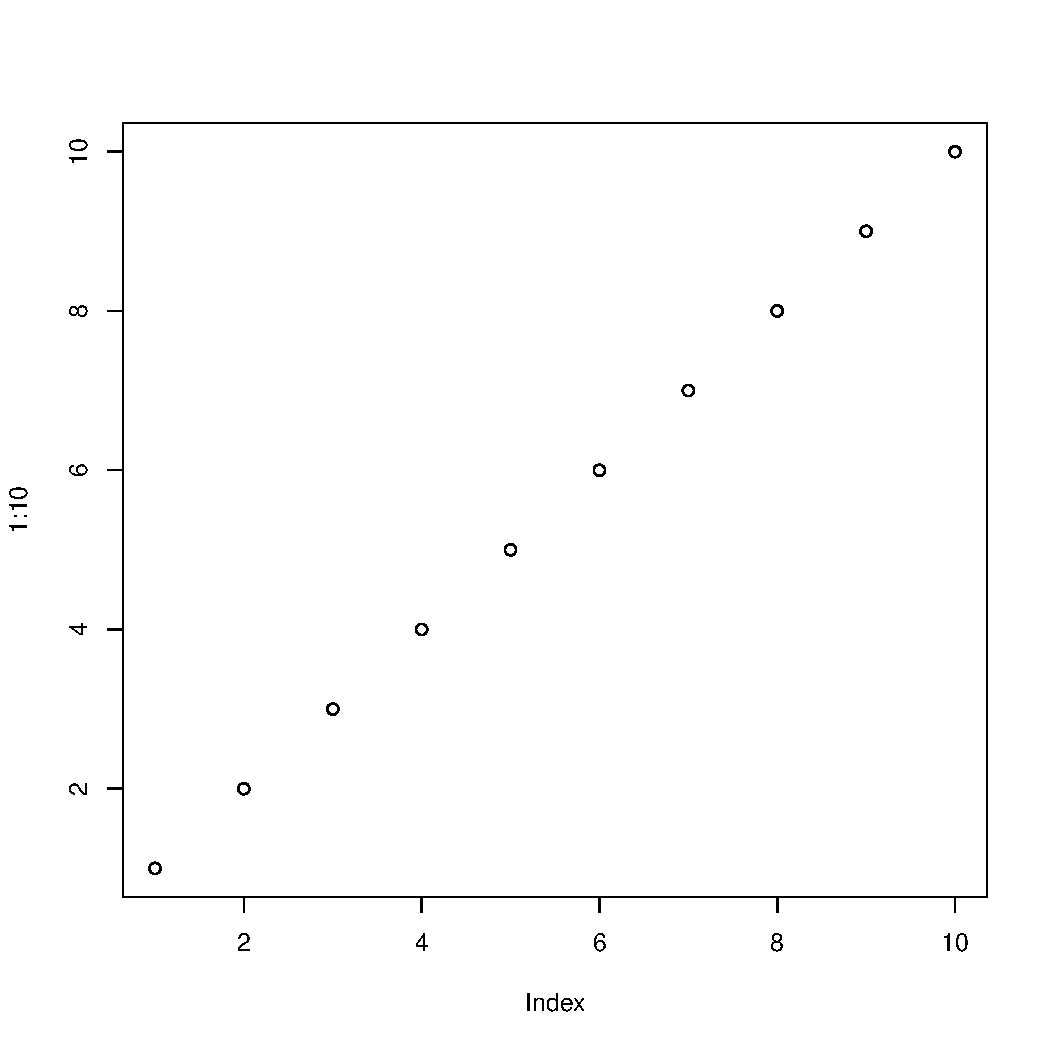
\includegraphics{NMF-vignette-heatmap_consensus_inc}
\caption{Heatmap of consensus matrix}
\label{fig:heatmap_consensus}
\end{figure}
    
\begin{figure}[ht]
\centering
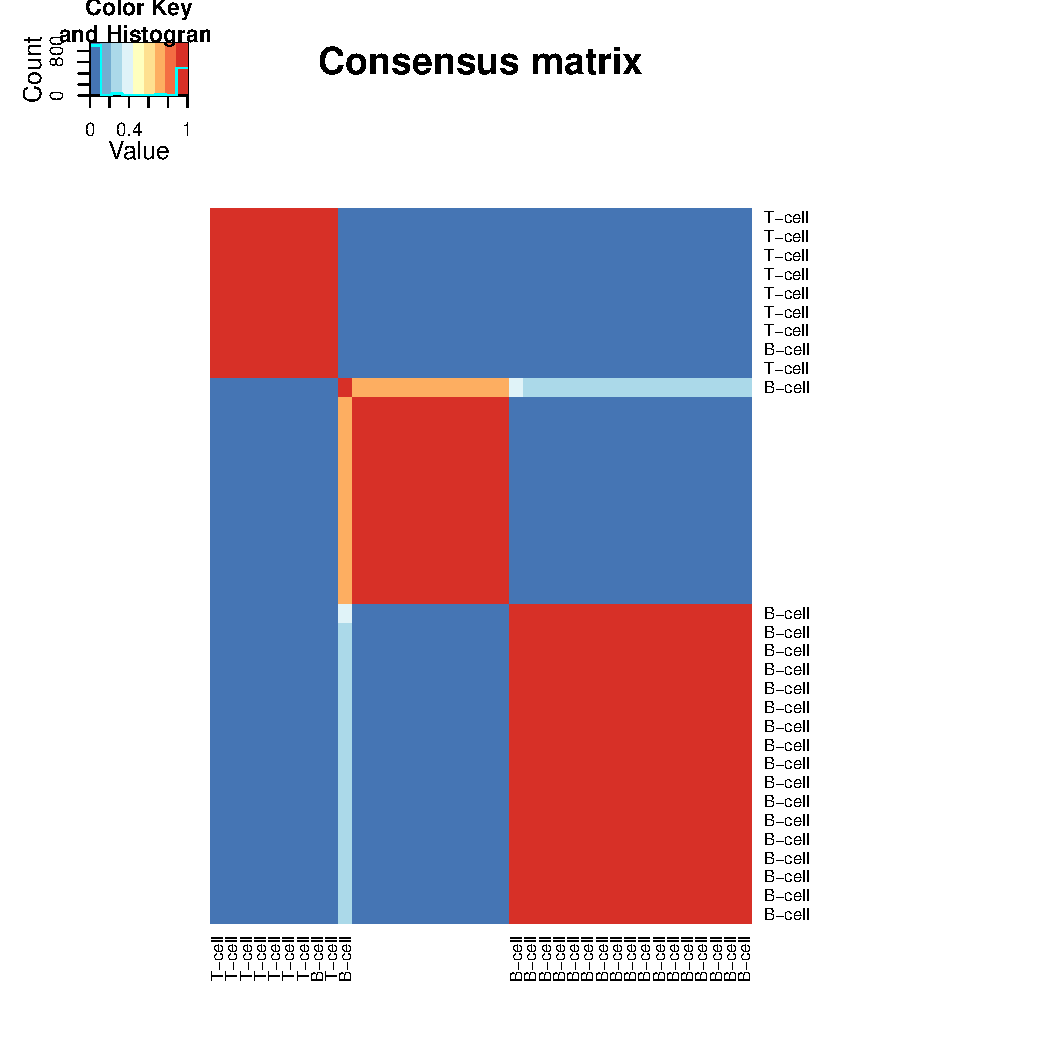
\includegraphics{consensus}
\caption{Heatmap of consensus matrix (100 runs of Brunet's algorithm on Golub
dataset)}
\label{fig:heatmap_consensus_precomp}
\end{figure}

\subsection{Comparing algorithms}
To compare the results from different algorithms, one can pass a list of methods 
in argument \code{method}. To enable a fair comparison, a deterministic seeding 
method should also be used. Here we fix the random seed to 123456. 

\begin{Schunk}
\begin{Sinput}
 res.multi.method <- nmf(esGolub, 3, list('brunet', 'lee', 'ns'), seed=123456)
\end{Sinput}
\end{Schunk}

Passing the result to method \code{compare} produces a \code{data.frame} 
that contains summary measures for each method. Again, prior knowledge of classes 
may be used to compute clustering quality measures:  

\begin{Schunk}
\begin{Sinput}
 compare(res.multi.method)
\end{Sinput}
\begin{Soutput}
       method   seed      metric rank sparseness.basis sparseness.coef
brunet brunet 123456        'KL'    3        0.6392676       0.6217884
lee       lee 123456 'euclidean'    3        0.7268875       0.4465608
nsNMF   nsNMF 123456        'KL'    3        0.6777185       0.7350386
         residuals niter  cpu cpu.all nrun
brunet    543535.7   510 0.56    0.56    1
lee    673513120.5  1780 1.87    1.87    1
nsNMF     585106.4   970 1.42    1.42    1
\end{Soutput}
\begin{Sinput}
 # If prior knowledge of classes is available
 compare(res.multi.method, class=esGolub$Cell)
\end{Sinput}
\begin{Soutput}
       method   seed      metric rank sparseness.basis sparseness.coef
brunet brunet 123456        'KL'    3        0.6392676       0.6217884
lee       lee 123456 'euclidean'    3        0.7268875       0.4465608
nsNMF   nsNMF 123456        'KL'    3        0.6777185       0.7350386
          purity   entropy   residuals niter  cpu cpu.all nrun
brunet 0.8157895 0.3926954    543535.7   510 0.56    0.56    1
lee    0.5789474 0.7231282 673513120.5  1780 1.87    1.87    1
nsNMF  0.7894737 0.4691212    585106.4   970 1.42    1.42    1
\end{Soutput}
\end{Schunk}

When the computation is performed with error tracking enabled, an error plot is 
produced by method \code{plot} (see figure \ref{fig:multi_error}):

\begin{Schunk}
\begin{Sinput}
 res <- nmf(esGolub, 3, list('brunet', 'lee', 'ns'), seed=123456, .options='t')
 plot(res)
\end{Sinput}
\end{Schunk}

\begin{figure}[ht]
\centering
\includegraphics{NMF-vignette-multiple_errorplot_include}
\caption{Error tracks comparing methods \texttt{'brunet', 'lee', 'nsNMF'}}
\label{fig:multi_error}
\end{figure}


 
\section{Extending the package}

We developed the \nmfpack\ package with the objective to facilitate the integration 
of new NMF methods, trying to impose only few requirements on their implementations. 
All the built-in algorithms and seeding methods are implemented as strategies 
that are called from within the main interface method \code{nmf}. 

The user can define new strategies and those are handled in exactly the same way as 
the built-in ones, benefiting from the same utility functions to interpret the 
results and assess their performance. 

\subsection{Custom algorithm}
%New NMF algrithms can be defined in two ways:
%
%\begin{itemize}
%\item as a single \code{function} 
%\item as a set of functions that implement a pre-defined \emph{iterative schema}
%\end{itemize}
%
%\subsubsection{Defined as a \code{function}}

\subsubsection{Using a custom algorithm}\label{sec:algo_custom}
To define a strategy, the user needs to provide a \code{function} that 
implements the complete algotihm. It must be of the form: 

\begin{Schunk}
\begin{Sinput}
 my.algorithm <- function(x, seed, param.1, param.2){
 	# do something with starting point
 	# ...
 	
 	# return updated starting point
 	return(seed)
 }
\end{Sinput}
\end{Schunk}
Where:

\begin{description}
\item[target] is a \code{matrix}; 
\item[start] is an object that inherits from class \code{NMF}. This \code{S4} 
class is used to handle NMF models (matrices \code{W} and \code{H}, objective 
function, etc\dots);
\item[param.1, param.2] are extra parameters specific to the algorithms;
\end{description}

The function must return an object that inherits from class \code{NMF}

For example:
\begin{Schunk}
\begin{Sinput}
 my.algorithm <- function(x, seed, scale.factor=1){
 	# do something with starting point
 	# ...
 	# for example: 
 	# 1. compute principal components	
 	pca <- prcomp(t(x), retx=TRUE)
 	
 	# 2. use the absolute values of the first PCs for the metagenes
 	# Note: the factorization rank is stored in object 'start'	
 	factorization.rank <- nbasis(seed)
 	metagenes(fit(seed)) <- abs(pca$rotation[,1:factorization.rank])
 	# use the rotated matrix to get the mixture coefficient
 	# use a scaling factor (just to illustrate the use of extra parameters)
 	metaprofiles(fit(seed)) <- t(abs(pca$x[,1:factorization.rank])) / scale.factor
 	
 	# return updated data
 	return(seed)
 }
\end{Sinput}
\end{Schunk}

To use the new method within the package framework, one pass \code{my.algorithm} 
to main interface \code{nmf} via argument \code{method}. Here we apply the 
algorithm to some matrix \code{V} randomly generated: 

\begin{Schunk}
\begin{Sinput}
 n <- 50; r <- 3; p <- 20
 V <-syntheticNMF(n, r, p, noise=TRUE)
\end{Sinput}
\end{Schunk}

\begin{Schunk}
\begin{Sinput}
 nmf(V, 3, my.algorithm, scale.factor=10)
\end{Sinput}
\begin{Soutput}
<Object of class: NMFfit >
 # Model:
  <Object of class: NMFstd >
  features: 50 
  basis/rank: 3 
  samples: 20 
 # Details:
  algorithm:  NMF.algo.2e75443d 
  seed:  random 
  distance metric:  'euclidean' 
  residuals:  637.5985 
  parameters:
  $scale.factor
  [1] 10
  
  Timing:
     user  system elapsed 
    0.000   0.000   0.003 
\end{Soutput}
\end{Schunk}

\subsubsection{Using a custom distance measure}
The default distance measure is based on the euclidean distance. 
If the algorithm is based on another distance measure, this one can be 
specified in argument \code{objective}, either as a \code{character} string 
corresponding to a built-in objective function, or a custom \code{function} 
definition:

\begin{Schunk}
\begin{Sinput}
 # based on Kullbach-Leibler divergence
 nmf(V, 3, my.algorithm, scale.factor=10, objective='KL')
\end{Sinput}
\begin{Soutput}
<Object of class: NMFfit >
 # Model:
  <Object of class: NMFstd >
  features: 50 
  basis/rank: 3 
  samples: 20 
 # Details:
  algorithm:  NMF.algo.2e7ccae3 
  seed:  random 
  distance metric:  'KL' 
  residuals:  1631.873 
  parameters:
  $scale.factor
  [1] 10
  
  Timing:
     user  system elapsed 
    0.000   0.000   0.002 
\end{Soutput}
\begin{Sinput}
 # based on custom distance metric
 nmf(V, 3, my.algorithm, scale.factor=10
 	, objective=function(target, x){ 
 			( sum( (target-fitted(x))^4 ) )^{1/4} 
 		}
 )
\end{Sinput}
\begin{Soutput}
<Object of class: NMFfit >
 # Model:
  <Object of class: NMFstd >
  features: 50 
  basis/rank: 3 
  samples: 20 
 # Details:
  algorithm:  NMF.algo.525681f8 
  seed:  random 
  distance metric:  <function> 
  residuals:  9.356993 
  parameters:
  $scale.factor
  [1] 10
  
  Timing:
     user  system elapsed 
    0.010   0.000   0.003 
\end{Soutput}
\end{Schunk}

%\subsubsection{Using the iterative schema} 
%
%NMF algorithms generally implement the following common iterative schema:
%
%\begin{enumerate}
%\item
%\item 
%\end{enumerate}

\subsubsection{Defining algorithms for mixed sign data}
All the algorithms implemented in the \nmfpack package assume that the input data is nonnegative.
However, some methods exist in the litterature that work with relaxed constraints, where 
the input data and one of the matrix factors ($W$ or $H$) are allowed to have negative 
entries (eg. semi-NMF \cite{Ding2008, Roux2008}).
Strictly speaking these methods do not fall into the NMF category, but still solve constrained matrix factorization 
problems, and could be considered as NMF methods when applied to non-negative data.
Moreover, we received user requests to enable the development of semi-NMF type methods within the package's framework.
Therefore, we designed the \nmfpack package so that such algorithms -- that handle negative data -- can be 
integrated. This section documents how to do it.

By default, as a safe-guard, the sign of the input data is checked before running any method, so that the 
\code{nmf} function throws an error if applied to data that contain negative entries
\footnote{Note that on the other side, the sign of the factors returned by the algorithms is never 
checked, so that one can always return factors with negative entries.}.
To extend the capabilities of the \nmfpack package in handling negative data, 
and plug mixed sign NMF methods into the framework, the user needs to specify the argument 
\code{mixed=TRUE} in the call to the \code{nmf} function.
This will skip the sign check of the input data and let the custom algorithm perform the factorization.
 
As an example, we reuse the previously defined custom algorithm\footnote{As it is defined here, the custom 
algorithm still returns nonnegative factors, which would not be desirable in a real example, as one would not 
be able to closely fit the negative entries.}:

\begin{Schunk}
\begin{Sinput}
 # put some negative input data 
 V.neg <- V; V.neg[1,] <- -1;
 # this generates an error
 err <- try( nmf(V.neg, 3, my.algorithm, scale.factor=10) )
 err
\end{Sinput}
\begin{Soutput}
[1] "Error in .local(x, rank, method, ...) : \n  Input matrix x contains some negative entries.\n"
attr(,"class")
[1] "try-error"
\end{Soutput}
\begin{Sinput}
 # this runs my.algorithm without error
 nmf(V.neg, 3, my.algorithm, mixed=TRUE, scale.factor=10)
\end{Sinput}
\begin{Soutput}
<Object of class: NMFfit >
 # Model:
  <Object of class: NMFstd >
  features: 50 
  basis/rank: 3 
  samples: 20 
 # Details:
  algorithm:  NMF.algo.76c48d24 
  seed:  random 
  distance metric:  'euclidean' 
  residuals:  639.6262 
  parameters:
  $scale.factor
  [1] 10
  
  Timing:
     user  system elapsed 
    0.000   0.000   0.003 
\end{Soutput}
\end{Schunk}

\subsubsection{Specifying the NMF model}
If not specified in the call, the NMF model that is used is the standard one, 
as defined in equation \refeqn{NMFstd}. However, some NMF algorithms have different 
underlying models, such as non-smooth NMF \cite{nsNMF2006} which uses an extra matrix factor 
that introduces an extra parameter, and change the way the target matrix is 
approximated.

The NMF models are defined as S4 classes that extends class \code{NMF}. All the 
available models can be retreived calling the \code{nmfModel()} function with no 
argument:

\begin{Schunk}
\begin{Sinput}
 nmfModel()
\end{Sinput}
\begin{Soutput}
[1] "NMFstd"    "NMFOffset" "NMFns"    
\end{Soutput}
\end{Schunk}
 
One can specify the NMF model to use with a custom algorithm, using argument 
\code{model}. Here we first adapt a bit the custom algorithm, to justify and 
illustrate the use of a different model.
We use model \code{NMFOffset} \cite{Badea2008}, that includes an offset to 
take into account genes that have constant expression levels accross the samples:

\begin{Schunk}
\begin{Sinput}
 my.algorithm.offset <- function(x, seed, scale.factor=1){
 	# do something with starting point
 	# ...
 	# for example: 
 	# 1. compute principal components	
 	pca <- prcomp(t(x), retx=TRUE)
 	
 	# retrieve the model being estimated
 	data.model <- fit(seed)
 	
 	# 2. use the absolute values of the first PCs for the metagenes
 	# Note: the factorization rank is stored in object 'start'	
 	factorization.rank <- nbasis(data.model)
 	metagenes(data.model) <- abs(pca$rotation[,1:factorization.rank])	
 	# use the rotated matrix to get the mixture coefficient
 	# use a scaling factor (just to illustrate the use of extra parameters)
 	metaprofiles(data.model) <- t(abs(pca$x[,1:factorization.rank])) / scale.factor
 	
 	# 3. Compute the offset as the mean expression
 	data.model@offset <- rowMeans(x)	
 	
 	# return updated data
 	fit(seed) <- data.model
 	seed
 }
\end{Sinput}
\end{Schunk}

Then run the algorithm specifying it needs model \code{NMFOffset}:
\begin{Schunk}
\begin{Sinput}
 # run custom algorithm with NMF model with offset
 nmf(V, 3, my.algorithm.offset, model='NMFOffset', scale.factor=10)
\end{Sinput}
\begin{Soutput}
<Object of class: NMFfit >
 # Model:
  <Object of class: NMFOffset >
  features: 50 
  basis/rank: 3 
  samples: 20 
  offset: [ 0.6761489 0.5007902 0.848937 0.3704305 0.8774585 ... ]
 # Details:
  algorithm:  NMF.algo.2f3c4a01 
  seed:  random 
  distance metric:  'euclidean' 
  residuals:  353.7908 
  parameters:
  $scale.factor
  [1] 10
  
  Timing:
     user  system elapsed 
    0.010   0.000   0.002 
\end{Soutput}
\end{Schunk}


\subsection{Custom seeding method}\label{sec:seed_custom}

The user can also define custom seeding method as a function of the form:


\begin{Schunk}
\begin{Sinput}
 # start: object of class NMF
 # target: the target matrix
 my.seeding.method <- function(model, target){
 	
 	# use only the largest columns for W
 	w.cols <- apply(target, 2, function(x) sqrt(sum(x^2)))
 	metagenes(model) <- target[,order(w.cols)[1:nbasis(model)]]
 	
 	# initialize H randomly
 	metaprofiles(model) <- matrix(runif(nbasis(model)*ncol(target))
 						, nbasis(model), ncol(target))
 
 	# return updated object
 	return(model)
 }
\end{Sinput}
\end{Schunk}

To use the new seeding method:
\begin{Schunk}
\begin{Sinput}
 nmf(V, 3, 'snmf/r', seed=my.seeding.method)
\end{Sinput}
\begin{Soutput}
<Object of class: NMFfit >
 # Model:
  <Object of class: NMFstd >
  features: 50 
  basis/rank: 3 
  samples: 20 
 # Details:
  algorithm:  snmf/r 
  seed:  NMF.seed.7eaf895c 
  distance metric:  'euclidean' 
  residuals:  154.3545 
  Iterations: 80 
  Timing:
     user  system elapsed 
    0.460   0.000   0.461 
\end{Soutput}
\end{Schunk}

\section{Advanced usage}

\subsection{Package specific options}
The package specific options can be retieved or changed using the \code{nmf.getOption} 
and \code{nmf.options} functions. 
These behave similarly as the \code{getOption} and \code{nmf.options} 
base functions:

\begin{Schunk}
\begin{Sinput}
 #show default algorithm and seeding method
 nmf.options('default.algorithm', 'default.seed')
 # retrieve a single option
 nmf.getOption('default.seed')
 # All options
 nmf.options()
\end{Sinput}
\end{Schunk}

Currently the following options are available:

% latex table generated in R 2.10.1 by xtable 1.5-6 package
% Wed Apr  7 15:27:05 2010
\begin{table}[ht]
\begin{center}
\begin{tabularx}{\textwidth}{>{\ttfamily}rlX}
  \hline
Option & Default value & Description\\ 
\hline
default.algorithm & brunet & Default NMF algorithm used by the \code{nmf} function when argument \code{method} is missing.
The value should the key of one of the available NMF algorithms. See \code{?nmfAlgorithm}.\\ 
track.interval & 30 & Number of iterations between two points in the residual track. 
This option is relevant only when residual tracking is enabled. See \code{?nmf}.\\ 
error.track & FALSE & Toggle default residual tracking. When \code{TRUE}, the \code{nmf} function 
compute and store the residual track in the result -- if not otherwise specified in argument \code{.options}.
Note that tracking may significantly slow down the computations.\\ 
default.seed & random & Default seeding method used by the \code{nmf} function when argument \code{seed} is missing.
The value should the key of one of the available seeding methods. See \code{?nmfSeed}.\\
parallel.backend & mc & Default parallel backend used used by the \code{nmf} function when argument \code{.pbackend} is missing.
Currently the following values are supported: \code{'mc'} for multicore, \code{'seq'} for sequential, \code{''} for \code{sapply}.\\
verbose & FALSE & Toggle verbosity.\\ 
debug & FALSE & Toggle debug mode, which is an extended verbose mode.\\ 
\hline
\end{tabularx}
\end{center}
\end{table}

 
\section{Session Info}
\begin{Schunk}
\begin{Soutput}
R version 2.11.1 (2010-05-31) 
x86_64-pc-linux-gnu 

locale:
 [1] LC_CTYPE=en_ZA.utf8       LC_NUMERIC=C             
 [3] LC_TIME=en_ZA.utf8        LC_COLLATE=en_ZA.utf8    
 [5] LC_MONETARY=C             LC_MESSAGES=en_ZA.utf8   
 [7] LC_PAPER=en_ZA.utf8       LC_NAME=C                
 [9] LC_ADDRESS=C              LC_TELEPHONE=C           
[11] LC_MEASUREMENT=en_ZA.utf8 LC_IDENTIFICATION=C      

attached base packages:
[1] tools     stats     graphics  grDevices utils     datasets  methods  
[8] base     

other attached packages:
 [1] RColorBrewer_1.0-2  synchronicity_1.0.9 bigmemory_4.2.3    
 [4] doMC_1.2.1          multicore_0.1-3     foreach_1.3.0      
 [7] codetools_0.2-2     iterators_1.0.3     xtable_1.5-6       
[10] NMF_0.4.9           Biobase_2.8.0      
\end{Soutput}
\end{Schunk}

\addcontentsline{toc}{section}{References}
\begin{thebibliography}{}

\bibitem[Albright {\em et al.}, 2006]{Albright2006} R. Albright, J. Cox, D. Duling, A. Langville, C. Meyer (2006).
\textbf{Algorithms, initializations, and convergence for the nonnegative matrix factorization}.
{\it NCSU Technical Report Math 81706}. \url{http://meyer.math.ncsu.edu/Meyer/Abstracts/Publications.html}.

\bibitem[Badea L., 2008]{Badea2008} Badea L. (2008). 
\textbf{Extracting Gene Expression Profiles Common to Colon and Pancreatic Adenocarcinoma Using Simultaneous Nonnegative Matrix Factorization}.
In \emph{Pacific Symposium on Biocomputing}, \emph{Volume 290} 2008:279--290.

\bibitem[Berry {\it et al}., 2006]{Berry06} Berry et al. (2006).
\textbf{Algorithms and Applications for Approximate Nonnegative Matrix Factorization}.
{\it Comput. Stat. Data Anal.}

\bibitem[Boutsidis and Gallopoulos, 2008]{Boutsidis2008}
Boutsidis C, Gallopoulos E.
\textbf{SVD based initialization: A head start for nonnegative matrix factorization}.
\emph{Pattern Recognition} 2008, 41:1350--1362,
\url{[http://linkinghub.elsevier.com/retrieve/pii/S0031320307004359]}.
Original \MATLAB code available from: \url{http://www.cs.rpi.edu/~boutsc/papers/paper1/nndsvd.m}

\bibitem[Brunet {\em et al.}, 2004]{Brunet04} Brunet, J.~P., Tamayo, P., Golub, T.~R., and Mesirov, J.~P. (2004).
\textbf{Metagenes and molecular pattern discovery using matrix factorization}.
{\em Proc Natl Acad Sci U S A\/}, {\bf 101}(12), 4164--4169.
Original \MATLAB code available from: \url{http://www.broadinstitute.org/cancer/pub/nmf}

\bibitem[A. Cichocki {\it et al}., 2004]{Cichocki04} Andrzej Cichocki , Rafal Zdunek, and Shun-ichi Amari (2004).
\textbf{New algorithms For Non-negative Matrix Factorization In Application To Blind Source Separation}.

\bibitem[Chu {\it et al.}, 2004]{Chu2004} M.T. Chu, F. Diele, R. Plemmons, S. Ragni.
\textbf{Optimality, computation, and interpretation of nonnegative matrix factorizations}.
{\it Technical Report}, Departments of Mathematics and Computer Science, Wake Forest University, USA.

\bibitem[Chris Ding {\em et al.}, 2008]{Ding2008} Ding, C., Li, T., Jordan, M.~I..
\textbf{Convex and Semi-Nonnegative Matrix Factorizations}.
\emph{IEEE Transactions on Pattern Analysis and Machine Intelligence}, 2008, vol. 32, no. 1, pp. 45-55
\url{[http://doi.ieeecomputersociety.org/10.1109/TPAMI.2008.277]}

\bibitem[doMC, 2009]{doMC}
{REvolution Computing}.
\textbf{doMC: Foreach parallel adaptor for the multicore package} 2009.
\url{[http://CRAN.R-project.org/package=doMC]}. [R package version 1.2.0].
  
  \bibitem[foreach, 2009]{foreach}
{REvolution Computing}. 
\textbf{doMC: Foreach parallel adaptor for the multicore package} 2009.
\url{[http://CRAN.R-project.org/package=doMC]}. [R package version 1.3.0].

\bibitem[Frigyesi and H\"{o}glund, 2008]{Frigyesi2008}
Frigyesi A, H\"{o}glund M: \textbf{Non-negative matrix factorization for the
  analysis of complex gene expression data: identification of clinically
  relevant tumor subtypes.} \emph{Cancer informatics} 2008,
  \textbf{6}:275--292,
  \url{[http://view.ncbi.nlm.nih.gov/pubmed/19259414]}.

\bibitem[Gao and Church, 2005]{Gao2005}
Gao Y, Church G: \textbf{Improving molecular cancer class discovery through
  sparse non-negative matrix factorization}. \emph{Bioinformatics} 2005,
  \textbf{21}(21):3970--3975,
  \url{[http://dx.doi.org/10.1093/bioinformatics/bti653]}.

\bibitem[Gentleman {\em et al.}, 2004]{Gentleman2004}
Gentleman RC, Carey VJ, Bates DM, Bolstad B, Dettling M, Dudoit S, Ellis B,
  Gautier L, Ge Y, Gentry J, Hornik K, Hothorn T, Huber W, Iacus S, Irizarry R,
  Leisch F, Li C, Maechler M, Rossini AJ, Sawitzki G, Smith C, Smyth G, Tierney
  L, Yang JYH, Zhang J: \textbf{{Bioconductor: open software development for
  computational biology and bioinformatics.}} \emph{Genome biology} 2004,
  \textbf{5}:R80,
  \url{[http://www.ncbi.nlm.nih.gov/pubmed/15461798]}.

\bibitem[Hutchins {\em et al.}, 2008]{Hutchins2008}
Hutchins LNN, Murphy SMM, Singh P, Graber JHH:
\textbf{Position-Dependent Motif Characterization Using Nonnegative Matrix Factorization.}
  \emph{Bioinformatics (Oxford, England)} 2008,
  \url{[http://view.ncbi.nlm.nih.gov/pubmed/18852176]}.

\bibitem[Kim and Park, 2007]{Kim2007}
Kim H, Park H.
\textbf{{Sparse non-negative matrix factorizations via alternating non-negativity-constrained least squares for microarray data analysis.}}
\emph{Bioinformatics (Oxford, England)} 2007,
\textbf{23}:1495--502,
\url{[http://www.ncbi.nlm.nih.gov/pubmed/17483501]}.
Original \MATLAB code available from: \url{http://www.cc.gatech.edu/~hpark/software/nmfsh_comb.m} 
and \url{http://www.cc.gatech.edu/~hpark/software/fcnnls.m}

\bibitem[Le Roux {\em et al.}, 2008]{Roux2008} Le Roux, J., de Cheveigné, A., Parra, L.~C.
\textbf{Adaptive Template Matching with Shift-Invariant Semi-NMF}. 
In {\it NIPS} 2008, 921-928.
\url{[http://dblp.uni-trier.de/db/conf/nips/nips2008.html#RouxCP08]} 

\bibitem[Lee and Seung, 2000]{Lee2000} Lee, D.~D. and Seung, H.~S. (2000).
\textbf{Algorithms for non-negative matrix factorization}.
In {\it {NIPS}\/}, 556-562.

\bibitem[Pascual-Montano {\em et al.}, 2006]{nsNMF2006} Pascual-Montano, A., Carazo, J.~M., Kochi, K., Lehmann, D., and Pascual-Marqui, R.~D. (2006).
\textbf{Nonsmooth nonnegative matrix factorization (nsnmf)}.
{\em IEEE transactions on pattern analysis and machine intelligence\/}, {\bf 28}(3), 403-415.

\bibitem[R Software, 2008]{R} R Development Core Team.
\textbf{R: A Language and Environment for Statistical Computing}.
Vienna, Austria. ISBN 3-900051-07-0.
\url{http://www.R-project.org}.

\bibitem[Zhang {\em et al.}, 2008]{Zhang2008}
Zhang J, Wei L, Feng X, Ma Z, Wang Y: 
\textbf{Pattern expression nonnegative matrix factorization: algorithm and applications to blind source separation}.
\emph{Computational intelligence and neuroscience} 2008,
\url{[http://view.ncbi.nlm.nih.gov/pubmed/18566689]}.


\end{thebibliography}


\end{document}
